\documentclass[a4paper,12pt]{report} %poner [twoside, 12pt] si lo vamos a imprimir

%-----------------------------------------|PAQUETES|-----------------------------------------
\usepackage{graphicx}
\usepackage{geometry} 
\usepackage{fancyhdr}
\usepackage[spanish]{babel}
\usepackage{pdfpages} 
\usepackage{verbatim}
\usepackage{amssymb}
\usepackage{tabularx}
\usepackage{parskip}
\usepackage{textcomp}
\usepackage{subfigure}
\usepackage[utf8]{inputenc}
\usepackage{float}
\usepackage{afterpage}
\usepackage{emptypage}
\usepackage{pdfpages}
%\usepackage{tikz}
%\usetikzlibrary{mindmap,trees}
\usepackage{amsmath}
%\usepackage{soul} %Para resaltar
%\usepackage{color} %Para resaltar
\usepackage{hyperref}
\usepackage{multicol}


%------------------------------|CONFIGURACION DE PAGINA Y MARGENES|-------------------------

%\pagestyle{fancy}
\geometry{
	a4paper,
	total={210mm,297mm},
	left=25mm,
	right=20mm,
	top=20mm,
	bottom=20mm}


%-----------------------------------------|ENCABEZADOS|-----------------------------------------
\pagestyle{fancy}
\fancyhf{}
\lhead{Mónaco - Ipóliti}
\rhead{\leftmark}
%\lfoot[\thepage]{}
%\rfoot[]{\thepage}
\cfoot{\thepage}

%----------------|CAMBIO NOMBRE "CAPITULO" POR "UNIDAD"|-------------------
%\addto\captionsspanish{\renewcommand{\chaptername}{Tarea}} 

%----------------|CAMBIO NOMBRE "CUADRO" POR "TABLA"|-------------------
\addto\captionsspanish{\renewcommand{\listtablename}{Índice de tablas}}
\addto\captionsspanish{\renewcommand{\tablename}{Tabla}}


\begin{document}
	
%-----------------------------------------|PORTADA EN PDF|-----------------------------------------
%\includepdf{caratula}
	


%-----------------------------------------|PORTADA CON TITELPAGE|-----------------------------------------
	 \begin{titlepage}
		\centering
		\vspace{1cm}
		{\bfseries\LARGE Universidad Tecnológica Nacional \par}
		\vspace{1cm}
		{
\includegraphics[scale=0.5]{Imagenes/logo}\par}
		\vspace{2cm}
		{\scshape\Large Facultad Regional Córdoba \par}
		\vspace{3cm}
		{\scshape\Huge Instrumentación para el Monitoreo de Redes de Telefonía Móvil \par}
		\vspace{3cm}
		{\itshape\Large Proyecto Fin de Grado \par}
		\vfill
		{\Large Autores: \par} %si borras el comando \par el nombre y la palabra autor quedan en la misma linea, de nada.
		{\Large Mónaco Mariano - Ipóliti Gino \par}
		{\Large 2020-2021 \par}
	\end{titlepage} 

	
	
%-----------------------------------------|INDICE|-----------------------------------------
\tableofcontents
\thispagestyle{empty}
\cleardoublepage
\setcounter{page}{1}

	
%-----------------------------------------|DOCUMENTO|-----------------------------------------
\section*{Prólogo}
Este documento fue creado para llevar en él las notas y los avances teóricos del proyecto final de grado. Formará parte del informe final.
Ademas de este documento llevamos una Bitácora (dos en realidad) donde vamos anotando hechos, tareas realizadas, problemáticas, ideas que surgen, dudas, etc. 
\thispagestyle{empty}

 \chapter{Definición de Requerimientos}
%\newpage

\textbf{20/07/2020 - Mariano}

\section{Generales \cite{gutierrez2020measurement}}

De manera \textbf{general} el instrumento debe ser capaz de extraer la información de una red LTE y procesarla para evaluar distintos aspectos de la red y del sistema en general.

(\textbf{Página interesante:}\url{https://www.sharetechnote.com/html/Handbook_LTE.html})

\begin{enumerate}
	\item Debe ser capaz de extraer información de redes LTE
	\item Procesar la información extraída de las redes LTE
	\item Las mediciones que debería poder realizar son:\footnote{Mediciones de capa física en transmisión de downlink mediante instrumentos de campo}
		\begin{enumerate}
			\item Mediciones de calidad de Radiofrecuencia:
				\begin{enumerate}
					\item Potencia y ancho de banda de canal
					\item Potencias en ON y OFF (sólo para frames TDD\footnote{TDD: Duplexación por división de tiempo})
					\item Emisiones fuera de banda
						\subitem Relación de fuga de canal adyacente
						\subitem Máscara de emisión espectral
					\item Piso de ruido en recepción: Interferencia en UL
				\end{enumerate}
			\item Mediciones de calidad de la modulación:
				\begin{enumerate}
					\item Magnitud de Error Vectorial (EVM\footnote{EVM: Magnitud del vector error}) pico y RMS
						\subitem Según canal: PBCH\footnote{Physical Broadcast Channel} (control), PDSCH\footnote{Physical Broadcast Channel} (datos), PCFICH\footnote{Physical Control Format Indicator Channel}, PSS\footnote{Primary Synchronization Signal}, SSS\footnote{Secondary Synchronization Signal}
						\subitem Según modulación: QPSK\footnote{Modulación por desplazamiento cuadrafásica}, 16QAM\footnote{Modulación de amplitud en cuadratura}, 64QAM
					\item Potencia de señales de soporte
						\subitem Señales de sincronismo: PSS y SSS
						\subitem Potencia en la señal de referencia (RS)
					\item Error o corrimiento de frecuencia
					\item Error de alineación de tiempo
				\end{enumerate}
		\end{enumerate}
\end{enumerate}


\textbf{28/07/2020 - Gino}

\section{Técnicos}

Especificaciones definidas por norma o necesarias y que se reflejan directamente en la selección del hardware.

\begin{enumerate}
	\item Bandas LTE \cite{bandas_lte} usadas en Argentina\footnote{Argentina está dentro de la ITU Region 2}:
	\begin{itemize}
		\item \textbf{Banda 2:} 1900 MHz (1850 MHz - 1990 MHz)
		\item \textbf{Banda 4:} 1700 MHz (1710 MHz - 2155 MHz)
		\item \textbf{Banda 5:} 850 MHz (824 MHz - 894 MHz)
		\item \textbf{Banda 7:} 2600 MHz (2500 MHz - 2690 MHz)
		\item \textbf{Banda 28:} 700 MHz (703 MHz - 803 MHz)
	\end{itemize}
	\item Todas las bandas utilizan el modo FDD\footnote{FDD: Frequency Division Duplexing}.
	\item Rango completo de frecuencias: 703 MHz a 2690 MHz.
	\item Anchos de banda posibles \textbf{[MHz]}: 1.4, 3, 5, 10, 15, 20.
\end{enumerate}


\chapter{Relevamiento de soluciones existentes}

\textbf{01/08/2020 - Gino}

\section{Anritsu BTS Master MT8220T \cite{anritsu}}

The BTS Master MT8220T Base Station Analyzer is the essential multi-function instrument for senior wireless technicians and RF engineers to accurately and quickly verify the installation and commissioning of base stations for optimal wireless network performance and for the on-going maintenance and troubleshooting to keep wireless network infrastructure fine-tuned.
The BTS Master MT8220T is small, lightweight and battery operated making it easy for the technician to use it anywhere at a cell site. With less than 5 minute warm-up time you get more useful battery life and you can start making measurements sooner. A GPS receiver is a standard feature allowing convenient mapping and triangulation of problematic interference signals in conjunction with Anritsu's interference hunting solutions.

\begin{figure}[H]
	\centering
	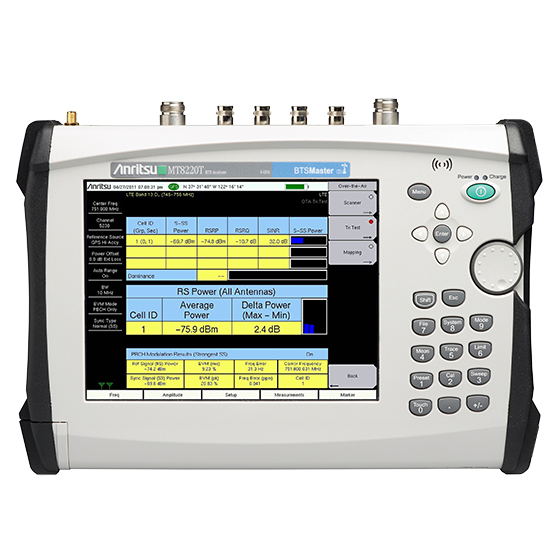
\includegraphics{Imagenes/anritsu1}
\end{figure}

%Cable and Antenna Analyzer
%\begin{itemize}
%	\item 400 MHz to 6 GHz
%	\item Measurements: RL, VSWR, Cable Loss, DTF, Phase (1- and 2-port), Gain
%	\item 2-port gain measurement uncertainty: < 0.45 dB
%	\item 2-port dynamic range: > 100 dB, typical 110 dB (400 MHz to 2800 MHz)
%	\item RF immunity: +17 dBm on-channel, +10 dBm on-frequency
%	\item Calibration: OSL and FlexCal™
%\end{itemize}
%
%Spectrum Analyzer
%\begin{itemize}
%	\item 150 kHz to 7.1 GHz
%	\item Measurements: Occupied Bandwidth, Channel Power, ACPR, C/I, Field Strength, Spectral Emissions, PIM Hunting
%	\item Dynamic range: > 95 dB in 1 Hz RBW
%	\item DANL: –163 dBm in 1 Hz RBW
%	\item Phase noise: –100 dBc/Hz @ 10 kHz offset
%	\item Frequency accuracy: ± 25 ppb with GPS On
%	\item Fast, Performance, No FFT and Burst Detect™ sweep modes
%\end{itemize}

Características
\begin{itemize}
	\item 2-port Cable and Antenna Analyzer 400 MHz to 6 GHz
	\item Spectrum Analyzer 150 kHz to 7.1 GHz
	\item Power Meter 10 MHz to 7.1 GHz
	\item GPS Receiver with Antenna
	\item Bias Tee
	\item High Accuracy Power Meter (up to 26 GHz with external sensor)
	\item Interference Analyzer with Mapping
	\item Channel Scanner
	\item Vector Signal Generator 400 MHz to 6 GHz
	\item Signal Analyzers
	\begin{itemize}
		\item LTE/LTE-A FDD/TDD, NB-IoT, W-CDMA/HSPA+,
		\item GSM/GPRS/EDGE, TD-SCDMA/HSPA+
		\item CDMA, EV-DO
		\item Fixed and Mobile WiMAX
	\end{itemize}
	\item CPRI\footnote{Common Public Radio Interface} RF Analyzer
	\item OBSAI RF Analyzer
	\item BBU Emulation
	\item PIM over CPRI
	\item eMBMS
	\item PIM\footnote{Passive Intermodulation} Alert (a downloadable easyTest™ script)
	\item Standard three-year warranty (battery one-year warranty)
\end{itemize}

\large{\textbf{Precio (desde): U\$D 16000 (usado)}}

\section{R\&S FSH Spectrum Analyzer \cite{fsh}}

The R\&S® FSH is a handheld spectrum analyzer and – depending on the model and the options installed – a power meter, a cable and antenna tester and a two-port vector network analyzer. It provides the most important RF analysis functions that an RF service technician or an installation and maintenance team needs to solve daily routine measurement tasks. For example, it can be used for maintaining or installing transmitter systems, checking cables and antennas, assessing signal quality in broadcasting, radiocommunications and service, measuring electric field strength or in simple lab applications. The R\&S® FSH can perform any of these tasks quickly, reliably and with high measurement accuracy. Weighing only 3 kg, the R\&S® FSH is a handy instrument.

\begin{figure}[H]
	\centering
	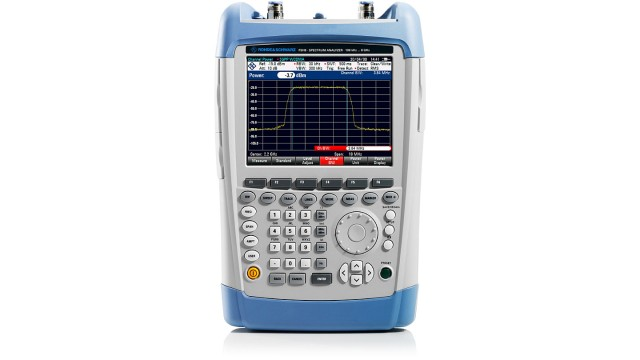
\includegraphics[scale=0.6]{Imagenes/FSH}
\end{figure}

\begin{itemize}
	\item Power measurements on pulsed signals
	\item Channel power measurements
	\item Adjacent channel power measurements
	\item Measurement of spurious emissions (spectrum emission mask)
	\item Measurement of the modulation spectrum on pulsed signals with gated sweep
	\item Analysis of transmit signals (connected to BTS or OTA)
	\begin{itemize}
		\item GSM/GPRS/EDGE
		\item WCDMA/HSDPA/HSPA+
		\item CDMA2000®
		\item 1xEV-DO
		\item LTE FDD/TDD
		\item NB-IoT
		\item TD-SCDMA/HSDPA
	\end{itemize}
	\item Vector network analysis
	\item One-port cable loss measurements
	\item Distance-to-fault measurements
	\item Vector voltmeter
	\item Position finding and increased measurement accuracy using the GPS receiver
\end{itemize}

\large{\textbf{Precio (desde): U\$D 10300}}

\chapter{Diseño de Arquitectura}

\section{Receptores - SDR} 

\textbf{21/04/21}

La radio definida por software (SDR)  hace uso de arquitecturas de hardware para DSP, microprocesadores, IC digitales especializados y software para producir señales moduladas para su transmisión y para su demodulación en el receptor. El receptor por software ideal muestreará y ditalizara las señales recibidas en la antena mediante un ADC y procesará la señal mediante el hardware de precesamiento elegido. En nuestro caso un microcontrolador de ST Electronics.

La mayoria de los receptores emplean la técnica de los receptores superheterodino: 

\begin{figure}[H]
	\centering
	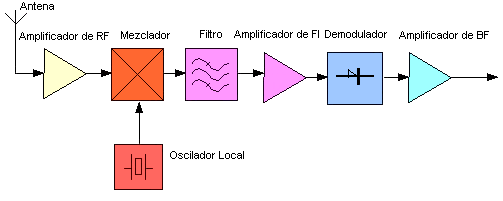
\includegraphics[scale=0.7]{Imagenes/Arquitectura/superhetero}
	\caption{Arquietecura de un receptor Superheterodino}
	\label{super}
\end{figure}

%-----> EXPLICAR MEZCLADORES ACA

El mezclador como sabemos es un circuito electrónico que hace uso de componentes no lineales para generar señales con frecuencias distintas a las de las señales de entrada. El objetivo de este bloque es desplazar en frecuencia una señal de interés para facilitar su manipulación. La nueva frecuencia a la que se lleva la señal en el receptor de la figura \ref{super} es la denominada Frecuencia Intermedia. Esto es de suma utilidad puesto que la electrónica de las etapas posteriores a esta se simplifica gracias a estar trabajando en esa frecuencia fija y ademas disponemos de dispositivos que a esa frecuencia intermedia tienen mas eficiencia, mas ganancia, Filtros mas selectivos, etc.

\begin{figure}[H]
	\centering
	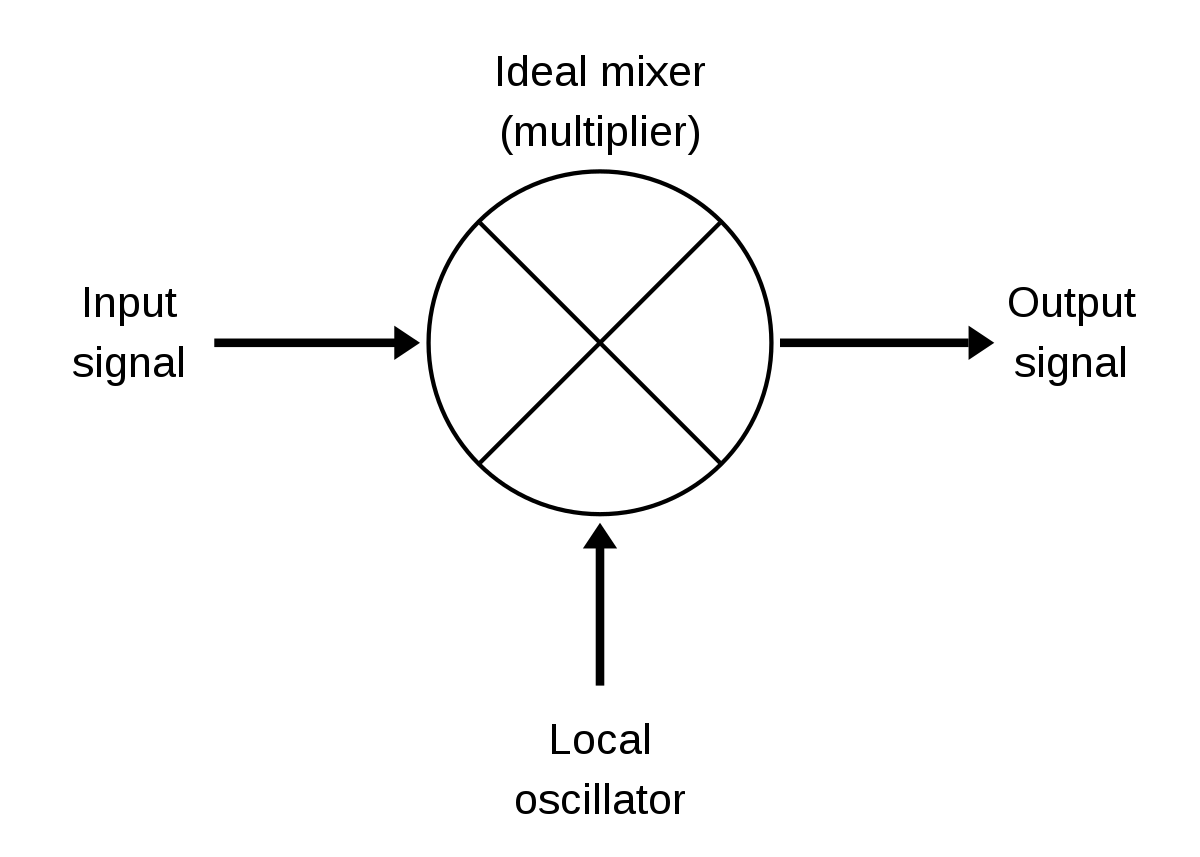
\includegraphics[scale=0.15]{Imagenes/Arquitectura/mixer}
	\caption{Mezclador}
	\label{mixer}
\end{figure}

Clasicamente encontramos 3 topologias:

\textbf{Mezclador desbalanceado:} Ademas de proporcinar el producto de las señales de entrada, deja que estas pasen y sean parte de la salida.

\textbf{Mezclador balanceado simple:} Una de las entradas es aplicada a un circuito con entrada diferencial lo que produce la supresión de esa señal a la salida, puede ser la del oscilador local o la señal de RF.

\textbf{Mezclador balanceado doble:} Anologo al anterior pero con sus dos entradas aplicadas a circuitos diferenciales, es decir que ninunga de las entradas es componente de la salida. Solo se tiene como salida al producto.

\begin{figure}[H]
	\centering
	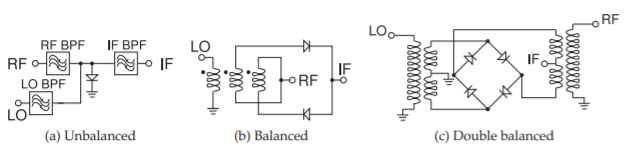
\includegraphics[scale=0.7]{Imagenes/Arquitectura/mixer-tipos}
	\caption{Topologias de mezcladores}
	\label{mixer-tipos}
\end{figure}  

% FIN EXPLCACIÓN MEZCLADORES

El tipo de demodulador o detector utilizado depende de la aplicación. En la mayoria de las arquitecturas de las radios definidas por software se utilizan los detectores en fase y cuadratura (I/Q) como el siguiente: 

\begin{figure}[H]
	\centering
	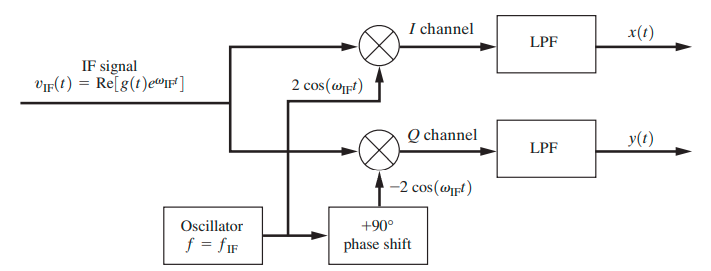
\includegraphics[scale=0.6]{Imagenes/Arquitectura/iq}
	\caption{Detector de IQ}
	\label{iq}
\end{figure}

%-----> EXPLICAR SEÑALES I/Q ACA

Para entender la modulación y demodulación por cuadratrura hay que saber, en primera instancia, que significa que dos señales estén en cuadratura.

Entonces, decimos que dos señales se encuentran en cuadratura cuando entre ellas existe una diferencia de fase de 90°, tal como se muestra aquí: 

\begin{figure}[H]
	\centering
	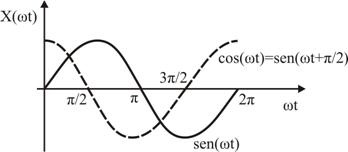
\includegraphics[scale=0.8]{Imagenes/Arquitectura/cuadratura}
	\caption{Señales en cuadratura}
	\label{cuad}
\end{figure}

Entonces disponemos de una señal ``en fase'' (Cos) y la otra ``en cuadratura'' (Sen). Se denomina ``I'' a la amplitud de la primera y ``Q'' a la amplitud de la segunda. De esta manera se puede expresar: 

\begin{center}
	$I\cdot\cos(2\cdot\pi\cdot f\cdot t)$
	
	$Q\cdot\sin(2\cdot\pi\cdot f\cdot t)$
\end{center}

Si sumamos estas señales obtendremos una señal que tiene propiedades interesantes: 

\begin{itemize}
	\item Si I y Q varian de igual manera, la amplitud de la señal resultante variará de manera proporcional.
	\item Si I y Q varian de manera diferente, se producirá desplazamientos de fase en la señal resultante luego de la suma.
\end{itemize}

Es decir que modificando los parámetros básicos de las señales en cuadratura podemos generar cualquier tipo de señal modulada, puesto que podemos modificar Amplitud, fase y frecuencia de la señal que resulta de la suma de las anteriores.

Una forma de ver esto de manera clara es con un \textbf{diagrama de fasores} como el de la figura \ref{fasores}

\begin{figure}[H]
	\centering
	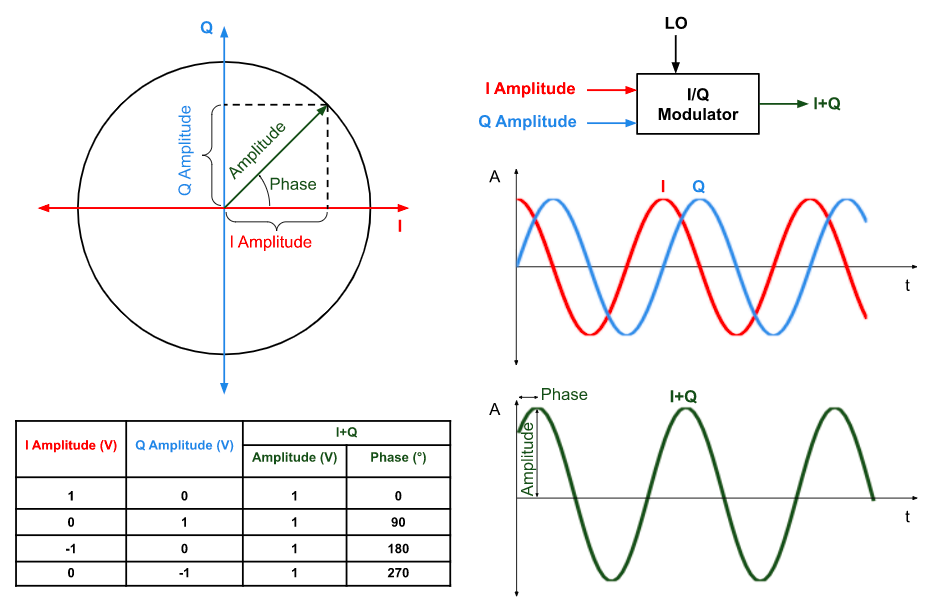
\includegraphics[scale=0.5]{Imagenes/Arquitectura/fasores}
	\caption{Graficos ilustrativos señales I/Q}
	\label{fasores}
\end{figure}

Entonces supongamos que queremos realizar una modulación digital QPSK. Lo hariamos como muestra el diagrama en bloques de la figura \ref{QPSK} y las señales se comportarian como se ve en la figura \ref{señalesqpsk}

\begin{figure}[H]
	\centering
	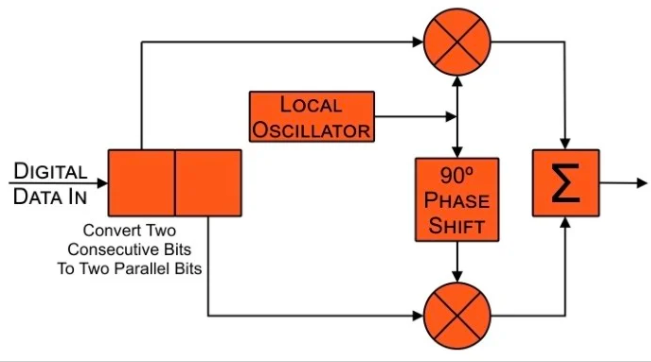
\includegraphics[scale=0.5]{Imagenes/Arquitectura/QPSK}
	\caption{Diagrama en bloques para efectuar una modulación QPSK }
	\label{QPSK}
\end{figure}

\begin{figure}[H]
	\centering
	\includegraphics[scale=0.6]{Imagenes/Arquitectura/qpsk-señales}
	\caption{Modulación QPSK }
	\label{señalesqpsk}
\end{figure}

Cuyo diagrama fasorial es el siguiente: 

\begin{figure}[H]
	\centering
	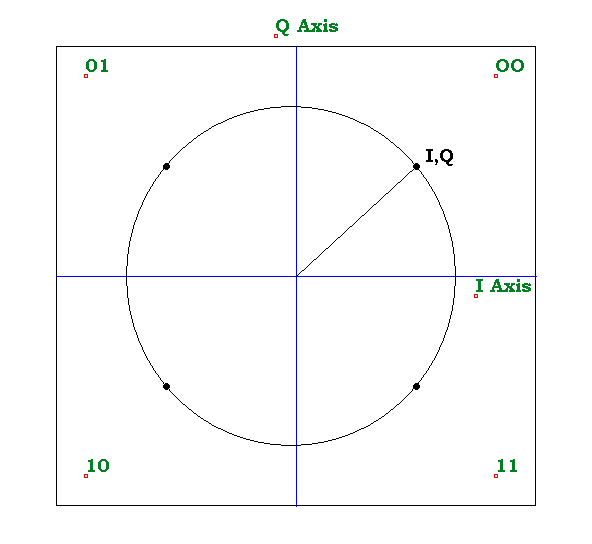
\includegraphics[scale=0.7]{Imagenes/Arquitectura/qpsk-fasores}
	\caption{QPSK en el dominio I-Q}
	\label{fasoresqpsk}
\end{figure}

Así, cualquier modulación tiene su representación en el dominio I-Q. Las señales $I(t)$ y $Q(t)$ en este caso son digitales pero pueden ser analógicas y efectuar otro tipo de modulación.

En cuanto a la demodulación, lo anterior resulta muy útil, vease la figura \ref{iqdemo}. \textbf{Las señales $I(t)$ y $Q(t)$ poseen la información suficiente para demodular cualquier tipo de modulación previa. Es por este motivo que resulta tan conveniente el uso en Radios Definidas por Software (SDR)}

\begin{figure}[H]
	\centering
	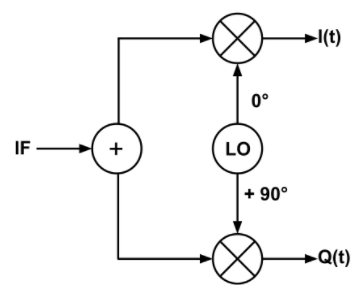
\includegraphics[scale=0.7]{Imagenes/Arquitectura/iqdemo}
	\caption{Demodulador I/Q}
	\label{iqdemo}
\end{figure}


%------- FIN EXPLICACIÓN IQ

Ahora bien, ¿que sucedería si la frecuencia del oscilador local de un receptor Superheterodino se ajusta de tal manera que se iguale a la frecuencia de la portadora ($f_{LO} = f_c$)?. Pues en este caso la frecuencia intermedia sería cero, o idealmente cero ($f_{IF} = 0$), y esto es lo que se denomina como un receptor de IF en cero o en ingles Zero-IF Receiver. En este caso el filtro de frecuencia intermedia (que se ven en la figura \ref{super}) se convierte en un filtro pasabajos (LPF). La combinación de un mezclador con un LPF funciona como detector de producto, por lo que no haría falta una etapa que proporcione un detector (como se ve en la figura \ref{super}); pero como nuestra necesidad es obtener las señales I/Q, se agrega un detector como el mostrado anteriormente (figura \ref{iq})

Los receptores de IF en cero poseen varias ventajas. El mismo hardware para el receptor de IF en cero puede utilizarse en muchas aplicaciones distintas para una manufactura económica. Debido a que se utiliza hardware de DSP, las características pasabanda de RF efectivas y las del detector se determinan mediante software para DSP. El software puede cambiarse fácilmente para satisfacer la aplicación deseada. El mismo hardware de IF en cero puede emplearse en receptores a diferentes bandas de VHF y UHF si se se selecciona la frecuencia del LO adecuada ($f_{LO} = f_c$) y si se sintoniza el filtro inicial, generalmente un circuito sintonizado a una sola frecuencia, a $f_c$.

El receptor de IF en cero posee la desventaja de una posible fuga de radiación del LO a través del puerto de entrada de antena debido a la vía de paso del mezclador. A su vez existirá un desplazamiento de DC en la salida del mezclador si existe una fuga en el LO a la entrada de antena, ya que una onda senoidal (señal del LO) multiplicada por sí misma produce un término de DC, además de una segunda armónica fuera de banda. Estos problemas se minimizarán con un mezclador balanceado de alta calidad y un blindaje en el LO. El receptor puede también poseer una figura pobre de ruido, ya que la circuitería de entrada generalmente no es una etapa de alta ganancia con bajo ruido. Como en cualquier otro receptor, el hardware debe diseñarse cuidadosamente para que exista un rango dinámico suficiente y prevenir que señales fuertes sobrecarguen al receptor, lo cual produce señales parásitas debido a las características no lineales, y que al mismo tiempo tenga una ganancia suficiente para la detección de señales débiles.







\textbf{29/07/2020 - Gino}

\section{Esquemas propuestos}

Los bloques con bordes discontinuos son aquellos opcionales o que no necesariamente deban estar en esa posición.

\subsection{Alternativa 1}

\begin{figure}[H]
	\centering
	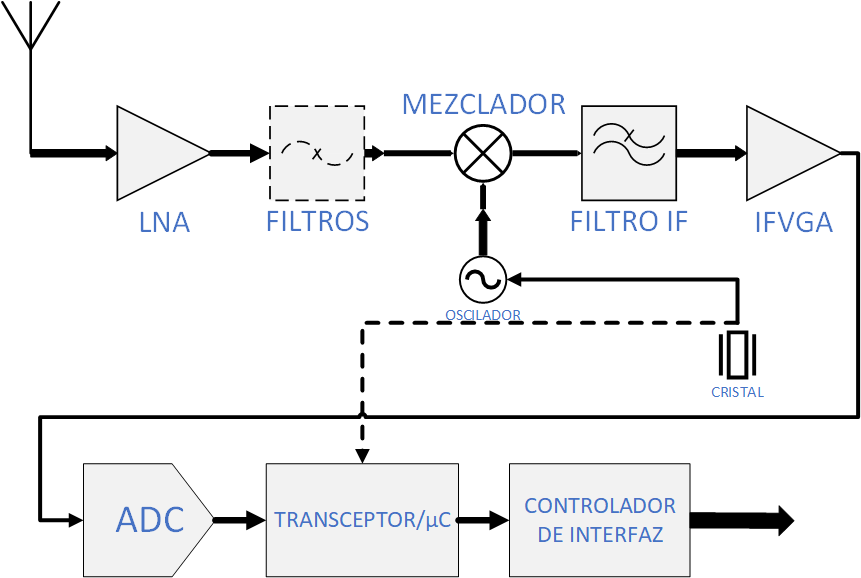
\includegraphics[scale=0.6]{Imagenes/Arquitectura/diagrama1}
\end{figure}

\subsection{Alternativa 2}

Las redes de adaptación pueden no ser necesarias. La más feasible es la segunda, ya que los transceptores suelen tener salidas diferenciales y es preferible tener una con terminación única en algunos casos.

\begin{figure}[H]
	\centering
	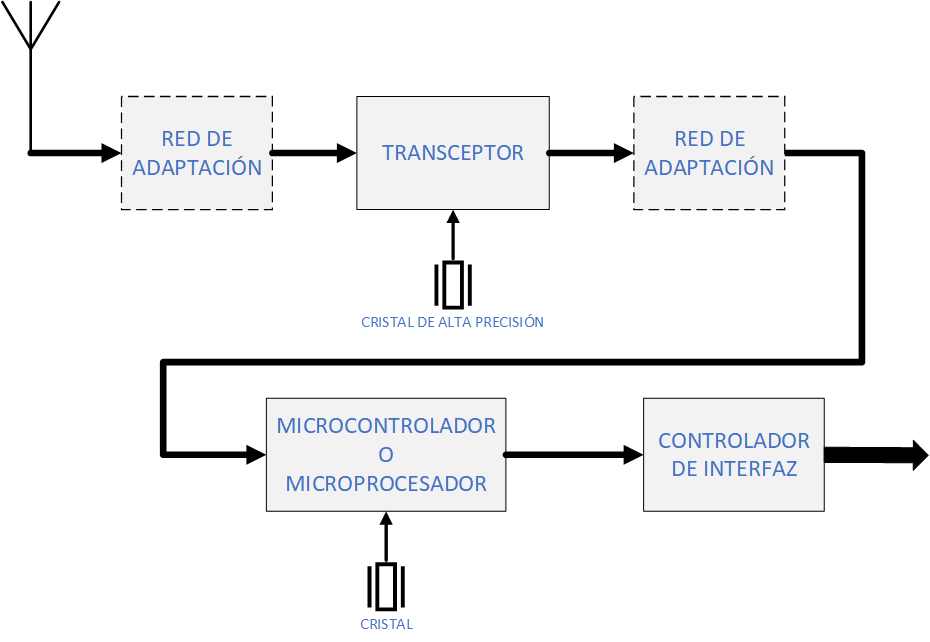
\includegraphics[scale=0.6]{Imagenes/Arquitectura/diagrama2}
\end{figure}

\textbf{03/08/2020 - Gino}
\subsection{Alternativa 3}

Esta bien podría ser la versión final de la arquitectura ya que se contemplan de forma general cada bloque necesario de un diseño típico de hardware SDR. Se supone que todas las interconexiones están adaptadas.

\begin{figure}[H]
	\centering
	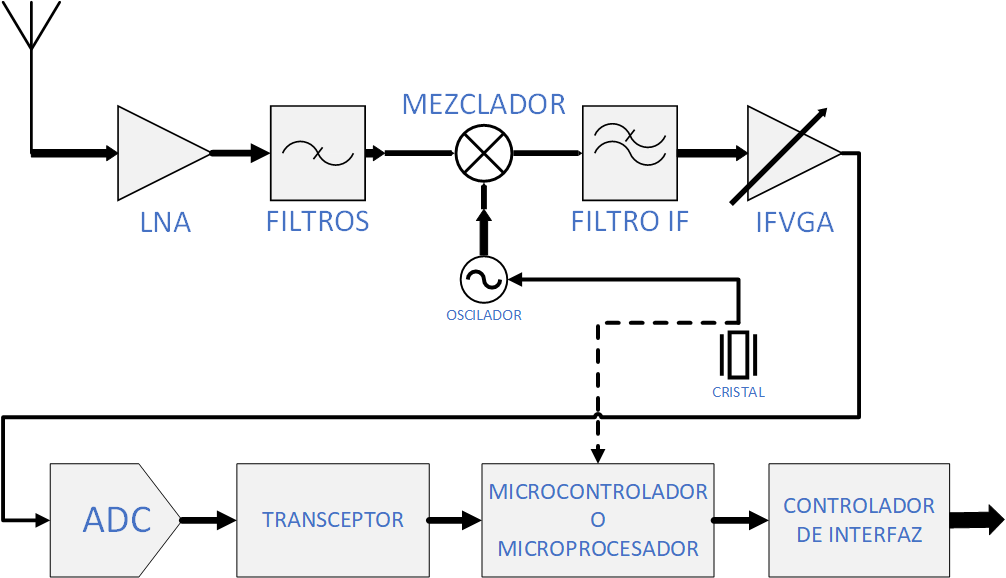
\includegraphics[scale=0.6]{Imagenes/Arquitectura/diagrama3}
\end{figure}

\textbf{29/07/20 Mariano}
\section{Transmisor y Receptor OFDM \cite{tesis}}

Los diagramas de la figura \ref{txrx} son implementaciones analógicas de transmisor y receptor de señales OFDM:

\begin{figure}[H]
	\centering
	\subfigure[Transmisor OFDM]{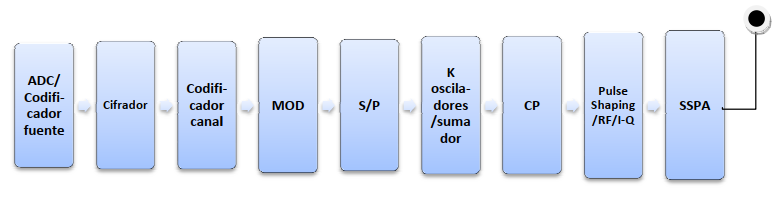
\includegraphics[scale=0.8]{Imagenes/Arquitectura/tx_ofdm} \label{tx_ofdm}}
	\subfigure[Receptor OFDM]{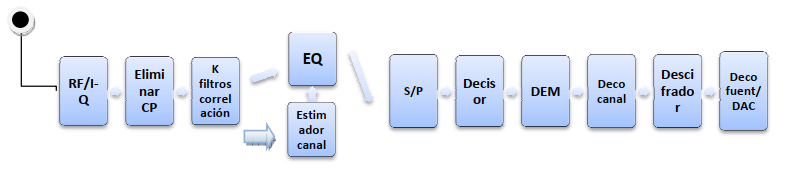
\includegraphics[scale=0.8]{Imagenes/Arquitectura/rx_ofdm}\label{rx_ofdm}}
	\caption{TX y RX OFDM ANALÓGICOS}
	\label{txrx}
\end{figure}

\subsection{Descripción del Transmisor}

\textbf{ADC / Codificador fuente:} Se encarga del muestreo y la cuantificación de la señal proveniente (normalmente) de una fuente adicional.

\textbf{Cifrador:} Incorpora algoritmos que proporcionan algún mecanismo de seguridad para la
comunicación a nivel de la capa física.

\textbf{Codificador de canal:} La codificación del canal se usa para solucionar el problema de requerir altos niveles de potencia de transmisión para lograr tasas de errores bajas. (Mas detalles en \cite{tesis}).

\textbf{Modulador:} Mapea el flujo binario entrante según un esquema de modulación digital convirtiéndolo a la salida en un flujo de símbolos complejos a una tasa $D_{serie}$ símbolos por segundo, o lo que es lo mismo con un tiempo de símbolo $T_{serie}$.

\textbf{Conversor serie/paralelo y Mapeador de subportadoras:} Demultiplexa el flujo de símbolos complejos en  símbolos paralelos haciendo corresponder, a continuación, un símbolo modulado serie a cada subportadora mediante
unas reglas determinadas de mapeo. El subflujo
de símbolos paralelo sale con una tasa $D = D_{serie}/K$ símbolos por segundo (con un
tiempo de símbolo $T = K\cdot T_{serie}$) y se denota mediante $S_{kl}$ , donde $k$ es el subíndice queindica la frecuencia de la subportadora que le corresponde, comprendido entre $k = ±1, ±2, ... , ±K/2$ (la componente DC suele dejarse vacía en sistemas prácticos debidoa motivos de implementación) y $l$ es el subíndice comprendido entre 0 y $L-1$ queindica el instante temporal en la transmisión.

\textbf{Banco de K filtros paso-banda paralelos $+$ sumador:} Esta etapa incorpora los osciladores y aparece solo en la versión analógica. Cada subflujo  a la salida del conversor S/P se hace pasar a través de un filtro
paso-banda. La señal a la salida de cada uno de estos filtros se suma, dando lugar a la señal
OFDM sin prefijo cíclico.
Como se detalla en el esquema digital, los osciladores se implementan mediante la FFT. (Para mas detalles de la versión analógica de este bloque dirigirse a \cite{tesis}).

\textbf{Incorporación del prefijo cíclico:} EL prefijo cíclico es es periodo que se añade entre símbolos para evitar, principalmente, la interferencia ínter-símbolos (ISI). En términos generales consiste en copiar una ultima parte del último símbolo y reproducirlo en este intervalo de guarda, como se ve en la figura \ref{CP}.

\begin{figure}[H]
	\centering
	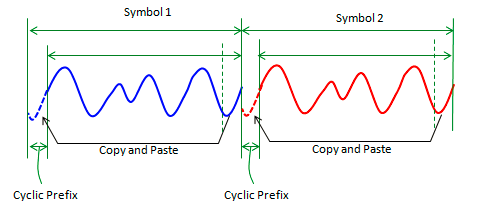
\includegraphics[scale=1]{imagenes/arquitectura/CP}
	\caption{Cyclic Prefix}
	\label{CP}
\end{figure}

Tras el sumador, se añade el prefijo cíclico y como consecuencia la duración del pulso es de $T_s = T + \Delta$. Como efecto no deseado, la incorporación del CP trae consigo una reducción de la eficiencia energetica y la tasa binaria transmitida.

\textbf{Oscilador RF y modulador IQ:} Consiste en un oscilador VCO o PLL que proporciona la portadora de la señal OFDM a frecuencia de UHF. Para que no haya una disminución de la SNR es muy importante que el oscilador en el transmisor y en le receptor estén sincronizados.

La portadora en fase se desfasa 90° obteniéndose la portadora en cuadratura. Ambas son multiplicadas respectivamente por la parte real e imaginaria de la señal OFDM.

\textbf{Amplificador de potencia:} Encargado de la amplificación de la señal para ser alimentada a la antena o a las L antenas.

\subsection{Descripción del Receptor} %Revisar conceptos

La señal recibida por la antena es bajada en frecuencia por un oscilador local que debe estar lo más adaptado posible al oscilador del transmisor. Aun así, los errores causados por desplazamiento en frecuencia y ruido de fase deben ser corregidos mediante técnicas de sincronización en frecuencia.





%--------------------------------
Como esta implementación (analógica) es costosa y un poco engorrosa se opta por una alternativa basada en el cálculo de la transformada discreta de Fourier mediante el algoritmo de la transformada Rápida de Fourier cuya eficiencia y facilidad de implementación fue la que permitió el éxito de OFDM. Esta alternativa digital se ve en la figura \ref{alt_dig}.

\begin{figure}[H]
	\centering
	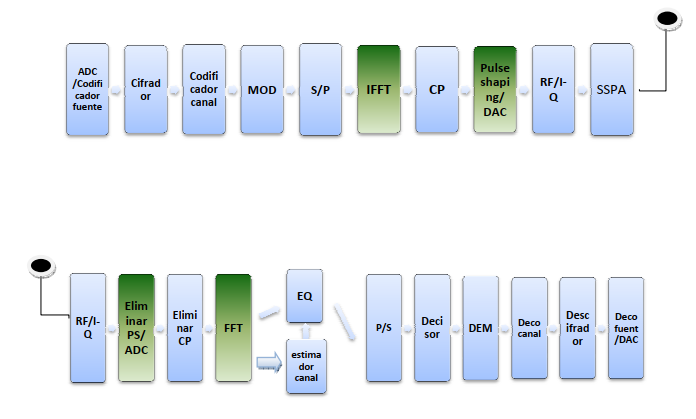
\includegraphics[scale=0.9]{Imagenes/Arquitectura/alt_dig}
	\caption{TX y RX OFDM DIGITALES}
	\label{alt_dig}
\end{figure}

En la figura \ref{alt_dig} los bloques en verde indican los cambios respecto al TX y RX analógico.


\chapter{Elección de componentes de cada bloque de la arquitectura}

\textbf{04/08/20 Mariano}

\section{Aspectos generales} \cite{sdr_engineers}

En lineas generales un SDR está conformado por las siguientes secciones:

\begin{itemize}
	\item Una sección analógica de RF (antena, filtros RF, multiplexores, LNA, atenuadores, mezcladores).
	\item Una sección analógica de Banda base (filtros analógicos, ADS y/o DAC).
	\item Unidades de procesamiento de señal (Filtros dentro del transceptor, FPGA o DSP, o procesadores de propósitos generales).
\end{itemize}

Para tener una referencia observamos el caso de PLUTO SDR. Las secciones anteriores, en esta plataforma especifica se ven conformadas por lo siguiente:

\begin{itemize}
	\item Una sección analógica de RF (antena, filtros RF, multiplexores, LNA, atenuadores, mezcladores)
		\subitem Antena y filtros de RF son responsabilidad del usuario.
		\subitem Los demás items (multiplexores, LNAs, atenuadores y mezcladores) están integrados en el transceptor AD9363.
		
	\item Una sección analógica de Banda base (filtros analógicos, ADS y/o DAC).
		\subitem Toda esta sección está implementada dentro del transceptor nombrado anteriormente.
		 
	\item Unidades de procesamiento de señal (Filtros dentro del transceptor, FPGA o DSP, o procesadores de propósitos generales). Esta sección se divide entre lo siguiente:
		\subitem Una parte es implementada en el AD9363. Esto  incluye los filtros de interpolación y diezmado de la banda media y los filtros FIR programables de 128 taps.
		\subitem Filtrados y diezmados opcionales se hacen con la FPGA Xilinx Zynq.
		\subitem La información I/Q pasa por el USB al host y de ahí se puede continuar procesándola con MATLAB.
\end{itemize}

\textbf{05/08/20 Gino}
\section{Transceptor}

\subsection{LMS6002D}

\url{https://limemicro.com/technology/lms6002d/}

Transceptor de Lime Microsystems con bajo costo (alrededor de \textbf{35 dólares}) dadas las prestaciones y comparado con otros integrados en el mismo segmento. 

\begin{itemize}
	\item Single chip transceiver
	\item Covers 300MHz to 3.8GHz
	\item Fully differential baseband signals
	\item Few external components
	\item Programmable modulation bandwidth: 1.5, 1.75, 2.5, 2.75, 3, 3.84, 5, 5.5, 6, 7, 8.75, 10, 12, 14, 20 and 28MHz
	\item Supports both FDD and TDD full duplex
	\item Integrated high performance 12-bit ADC and DAC
	\item Low voltage operation, 1.8V and 3.3V
	\item Standby current less than 1mA
	\item Tx RF output +6dBm, continuous wave
	\item 120 pin DQFN package
	\item Provision for Full Calibration
	\item Power down
	\item Serial interface
\end{itemize}

\subsection{AD9363}

\url{ttps://www.analog.com/en/products/ad9363.html#product-overview}

Transceptor de Analog Devices de costo medio (entre \textbf{60 y 120 dólares}). 

\begin{itemize}
	\item Radio frequency (RF) 2 × 2 transceiver with integrated 12-bit DACs and ADCs
	\item Wide bandwidth: 325 MHz to 3.8 GHz
	\item Supports time division duplex (TDD) and frequency division duplex (FDD) operation
	\item Tunable channel bandwidth (BW): up to 20 MHz
	\item Receivers: 6 differential or 12 single-ended inputs
	\item Superior receiver sensitivity with a noise figure: 3 dB
	\item Receive (Rx) gain control
	\begin{itemize}
		\item Real-time monitor and control signals for manual gain
		\item Independent automatic gain control (AGC)
	\end{itemize}
	\item Dual transmitters: 4 differential outputs
	\item Highly linear broadband transmitter
	\begin{itemize}
		\item Transmit (Tx) error vector magnitude (EVM): -34 dB
		\item Tx noise: $\leqslant-$157 dBm/Hz noise floor
		\item Tx monitor: 66 dB dynamic range with 1 dB accuracy
	\end{itemize}
	\item Integrated fractional N synthesizers
	\item 2.4 Hz local oscillator (LO) step size
	\item CMOS/LVDS digital interface
\end{itemize}

\subsection{NRF9160}

\url{https://www.nordicsemi.com/Products/Low-power-cellular-IoT/nRF9160}

Transceptor de Nordic Semiconductor. Tiene un costo bajo (\textbf{25 dólares} aproximadamente). La desventaja es que está diseñado para NB-IoT por ende los ancho de banda soportados son de 200 kHz y 1.4 MHz. Además, solo soporta frecuencias de entrada hasta los 2200 MHz, por lo que la banda 7 quedaría fuera. Lo bueno es que trae integrado un procesador Arm Cortex-M33 y existe software dedicado a monitoreo de enlaces LTE (\url{https://www.youtube.com/watch?v=m5V4Vo_Xemk})

\section{Cristales}
\subsection{MCU}
Para el STM32F723ZC se utilizará un cristal de 25 MHz como sugiere el fabricante. Los valores de los capacitores de carga se calculan de la siguiente manera:
\begin{equation}
	C_L = 2 \cdot (C_{Load\_cristal} - C_{parasita}\footnotemark)
\end{equation}
Para este caso:
\begin{align}
	C_{Load\_cristal} = 8 pF \\
	C_{parasita} = 2 pF \\
	C_L = 12 pF
\end{align}
\footnotetext{Capacitancia parásita del PCB.}

\chapter{Diseño del esquemático}
Consideraciones y/o detalles a tener en cuenta:
\begin{itemize}
	\item \textbf{Alimentación:}
	\begin{itemize}
		\item Se alimenta desde los 5v del puerto USB y se los reduce a 3,3v con un regulador.
		\item El ADC requiere 1,8v para las salidas digitales.
	\end{itemize}
	\item \textbf{Amplificador:}
	\begin{itemize}
		\item Se lo habilita por medio de switches de RF y se le controla la alimentación mediante un PMOS (high side switch).
	\end{itemize}
	\item \textbf{Mezclador:}
	\begin{itemize}
		\item Utiliza un bus serial propietario de 3-4 cables para su control y programación. Se elige el modo de 4 cables y se lo controla por SPI.
		\item Si no se usa un resonador dedicado, la señal de clock (referencia externa) debe tener una amplitud de 0,5 a 1,5 Vpp. Se debe acondicionar (3,3v $\rightarrow$ 1,5v).
	\end{itemize}	
	\item \textbf{ADC:}	 
	\begin{itemize}
		\item 2 canales (A y B), se usarán para muestras I y Q respectivamente. Entrega los datos de forma paralela y con el pin de A/\={B} se le indica al MCU que canal está presente.
		\item Tasa de muestreo hasta los 45 Msps, por lo que se puede reducir disminuyendo la frecuencia del clock.
	\end{itemize}
	\item \textbf{Transceptor:}
	\begin{itemize}
		\item Sólo se utilizará para recepción. No se encontró otro IC que fuese solo receptor y cumpliese con los requisitos.
	\end{itemize}
	\item \textbf{Microcontrolador:}
	\begin{itemize}
		\item Se utilizará la conectividad USB HS para asegurar la mayor velocidad de transferencia de datos hacia el host (PC).
		\item Controla el mezclador y transceptor por SPI1.
		\item Se deja la opción de agregarle una memoria flash externa y controlable por SPI4.
		\item Se programa por la interfaz JTAG de ARM.
		\item Toda señal de control para cualquier componente proviene del MCU.
	\end{itemize}
	\item \textbf{Generador de clock:}
	\begin{itemize}
		\item Idealmente se utiliza uno para proveer de señales de clock a todos los componentes que lo requieran.
		\item Si no se consigue entonces se deberán utilizar cristales individuales.
	\end{itemize}
\end{itemize}


\chapter{Elaboración del PCB}
\textbf{19/04/21 Mariano}

\section{Longitud critica $L_c$}

Se debe tener especial cuidado cuando la longitud de la pista supera una fracción de la longitud de onda de la señal que viaja por dicha pista. Esta fracción viene determinada por dos ecuación según no refiramos a Microstrip o Stripline:


\textbf{Stripline (trazo interno)}
\begin{equation}
L_c = \frac{c}{f} \cdot \frac{1}{\sqrt{\epsilon_r}} \cdot \frac{1}{12}
\end{equation}

Donde $\epsilon_r$ es la constante dieléctrica (o también llamada permitividad relativa del dieléctrico). $c$ se corresponde con la velocidad de la luz y $f$ es la frecuencia de interés.

\textbf{Microstrip (trazo externo)}
\begin{equation}
L_c = \frac{c}{f} \cdot \frac{1}{\sqrt{\epsilon_{ff}}} \cdot \frac{1}{12}
\end{equation}

$\epsilon_{ff}$ es la constante dielectrica efectiva. Usualmente este valor es menor que $\epsilon_r$ y la diferencia radica en que por encima de un trazo externo se encuentra el aire, entonces la constante es una resultante de dos medios dieléctricos.
Hay herramientas en la web que facilitan este calculo. Como ejemplo tenemos la siguiente herramienta: 

\url{https://www.pasternack.com/t-calculator-microstrip.aspx}

Cuyos datos los extraemos de: \url{https://jlcpcb.com/quote/pcbOrderFaq/PCB\%20Stackup} quien posiblemente sea nuestro proveedor. 


Para nuestro caso entonces este calculo nos arroja el siguiente resultado: 

$\epsilon_{ff} = 3,394$

Por lo tanto la longitud critica considerando una frecuencia máxima de 2700 Mhz: 

\begin{equation}
L_c = \frac{c}{f} \cdot \frac{1}{\sqrt{\epsilon_{ff}}} \cdot \frac{1}{12} = 0.5026 [cm]
\end{equation}


Es decir que la longitud de la pista por la cual circula una señal de 2700 Mhz como máximo, no puede superar los 5 mm.


\section{Consideraciónes para el uso efectivo de las 4 capas}

Típicamete las dos capas interiores se usan como plano de tierra (GND) y Alimentación (PWR). Entonces el ruteo se hará con "microstrip lines". Es decir quedaría, de manera muy general, algo así: 

\begin{enumerate}
	\item Trazado de pistas
	\item GND
	\item Trazado pistas PWR
	\item Trazado de pistas
\end{enumerate}

\section{Control de Impedancia de las pistas}

\url{https://cart.jlcpcb.com/impedance}

Del link anterior extraemos los datos para utilizarlos en la calculadora que el programa de diseño (KiCad) nos proporciona.

Es menester aclarar que se concidera para el calculo la utilización de Microstrip.

KiCad nos arroja el siguiente resultado: 

\begin{figure}[H]
	\centering
	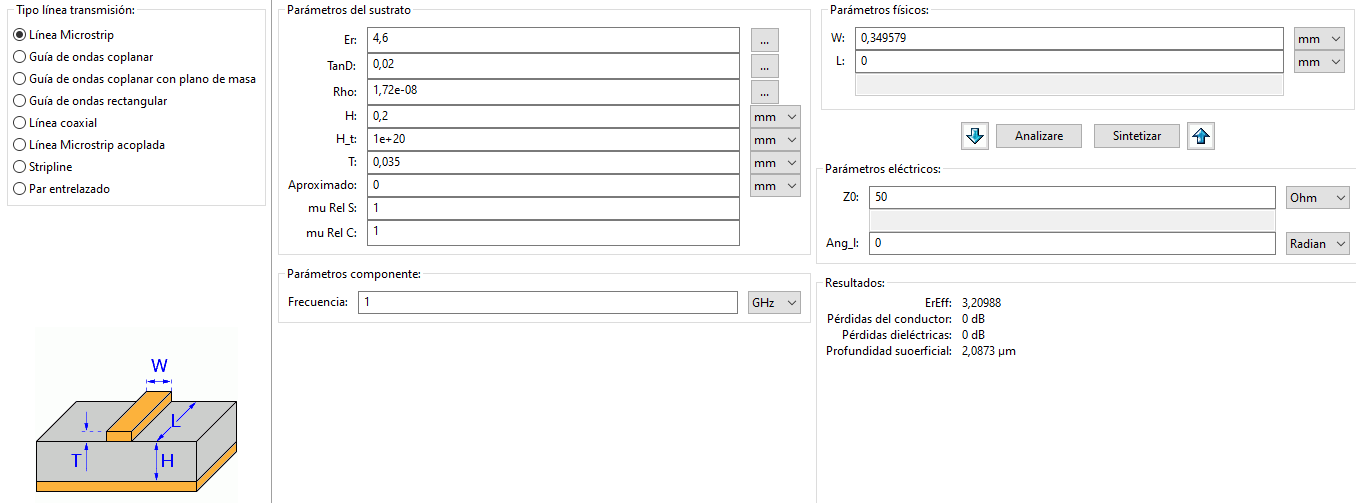
\includegraphics[scale=0.4]{Imagenes/PCB/impedancia_kicad}
	\caption{Ancho de pista para una impedancia de 50 ohm}
	\label{impedancia1}
\end{figure}

Pero el fabricante JLCPCB tiene su propia calculadora, esta herramienta arroja los siguientes resutados para los distintos valoes de impedancia y configuraciones (terminación única o diferencial): 

\begin{table} [H]
	\begin{center}
		\begin{tabular}{|c|c|c|c|c|}
			\hline
			\multicolumn{5}{|c|}{Longitudes en [mill] para distintos valores de impedancia} \\ \hline
			Impedancia		& 45 	& 90 	& 50 	& 100 \\ \hline
			T única			& 14,04	& X		& 11,55	& X \\ \hline
			T Diferencial	& X		& 10,28 & X		& 8,08 \\ \hline
		\end{tabular}
	\caption{Anchos de pistas (valores en [mill])}
	\label{impedancias}
	\end{center}
\end{table}


La ecuación \ref{ancho} es la que se utiliza para el calculo de los valores mostrados en la tabla \ref{impedancias}

\begin{equation}
w = h \cdot [\frac{1}{Z_0 \cdot C \cdot \epsilon_0 \cdot \epsilon_r} -2]
\label{ancho}
\end{equation}

Los parametros del material son: 

\begin{table} [H]
	\begin{center}
		\begin{tabular}{|c||c|}
			\hline
%			\multicolumn{5}{|c|}{Longitudes en [mill] para distintos valores de impedancia} \\ \hline
			Producto		& JLC7628  \\ \hline
			N° de capas			& 4	 \\ \hline
			Grosor	& 1,6 [mm]		\\ \hline
			Tipo de pista & Microstrip (pistas externas) \\ \hline
			Separación entre pistas T Diferencial & 8 [mills] \\ \hline
		\end{tabular}
		\caption{Parametros del producto}
		\label{placa}
	\end{center}
\end{table}


\section{Discontinuidades de impedancia}

Cuando algún trazo/pista culmina en un pad o algo que hace variar el ancho de la pista, se produce un cambio en la impedancia. Varios articulos leidos y experiencias de personas que diseñaron placas cuyas señales involucradas eran de alta frecuencia indican que esos cambios si bien son innegables, no afectan al desempeño, por lo cual no son tomados en cuenta. Solo en algunos casos particulares se intenta hacer un cambio progresivo del trazo para que no sea abrupto, nada más. 

\section{Clearance}

De manera general, en todos los casos se recomienda que las secciones de RF, antenna, alimentación y sección digital se mantengan separadas, especialmente la sección digital de la de RF. Para evitar que estas secciones interfieran entre ellas.

\section{Antennas and Bias Tee}

No lo tenemos implementado en nuestra placa.

\section{Thermal Vias}

Siguiendo la nota de aplicación AN1151\cite{thvias} de Diodes Incorporated sobre diseño de vias termales para encapsulados TQFN se obtuvieron los siguientes valores.

RFFC5072:
\begin{equation}
	N_{vias} = \left(\frac{3.71mm}{1.2mm}\right)^2 \approxeq 9
\end{equation}

MAX2837:
\begin{equation}
	N_{vias} = \left(\frac{4.57mm}{1mm}\right)^2 = 20.88 \rightarrow 16
\end{equation}

MAX1193:
\begin{equation}
	N_{vias} = \left(\frac{3.35mm}{1.1mm}\right)^2 \approxeq 9
\end{equation}

5P49V5929:
\begin{equation}
	N_{vias} = \left(\frac{2.8mm}{1.25mm}\right)^2 = 5.01 \rightarrow 4
\end{equation}

\chapter{Programación del Microcontrolador}


\textbf{Enlaces de utilidad:}

\url{https://www.youtube.com/watch?v=GZqwrcGNHO0&list=PLvHxU_pY8Jf9NYhzMauKIc2iBP5HGPYSM}

\url{https://www.youtube.com/watch?v=E8JpLtMlokw&list=PL1Hs_F1k2mdTwlGSv7lglkF_LtY0125OB&index=1}

\section{Arquitectura ARM}

\subsection{Introducción - generalidades}

Incluir aquí: 

Definición arquitectura ARM

Objetivo de los Cortex-M sistemas embebidos


\subsection{CISC-RISC}

La siguiente tabla resume las principales diferencias de cada una de las arquitecturas. Claramente en la bibliografia dedicada a este tema se puede encontrar mucha mas información si se desea, pero aquí se resalta las diferencias mas predominantes.

\begin{figure}[H]
	\centering
	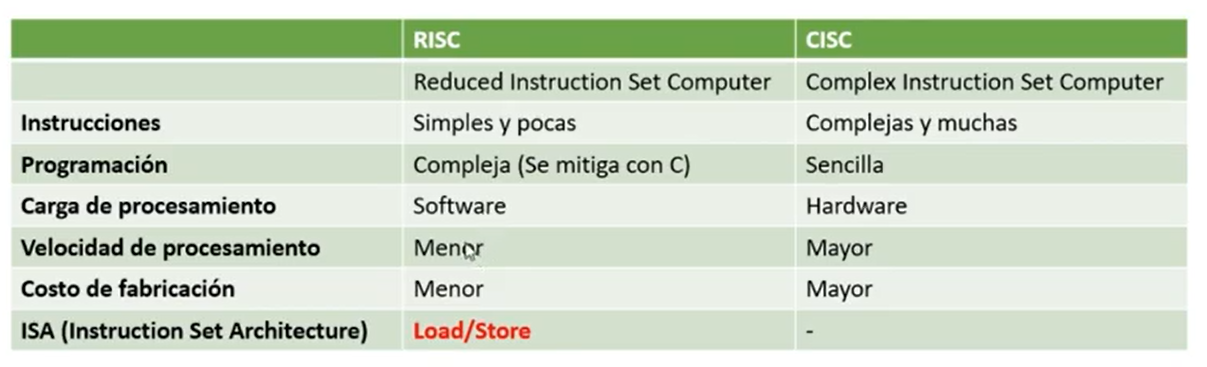
\includegraphics[scale=0.45]{Imagenes/stm/risc-cisc}
	\caption{RISC vs CISC}
	\label{cr}
\end{figure}


\subsection{Distribución de la memoria}

La distribución de la memoria no es universal y cambia según estemos usando un Microcontrolador que haga uso de un Cortex-M, Cortex-R o algún otro. Se muestra a continuación la organización de la memoria de los microcontroladores cuyo procesador sea un Cortex-M:



\begin{figure}[H]
	\centering
	\subfigure[Estructura general]{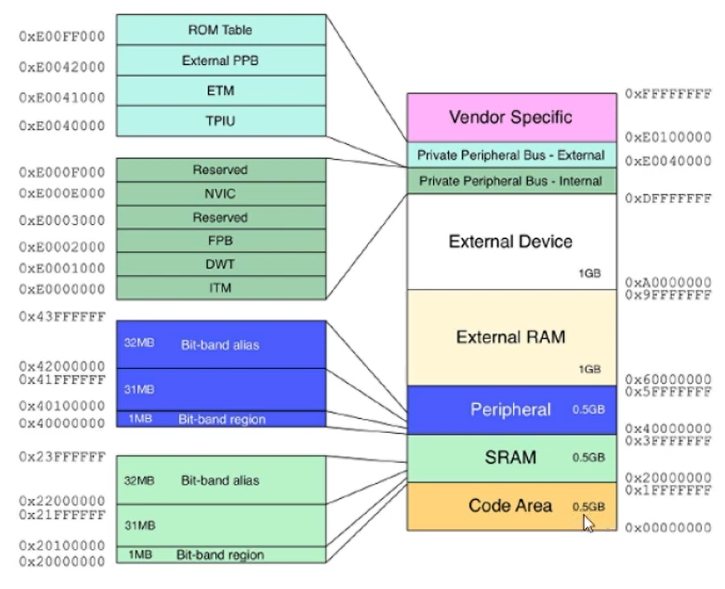
\includegraphics[scale=0.35]{Imagenes/stm/memoria1} \label{memo1}}
	\subfigure[Estructura de memoria del area de código]{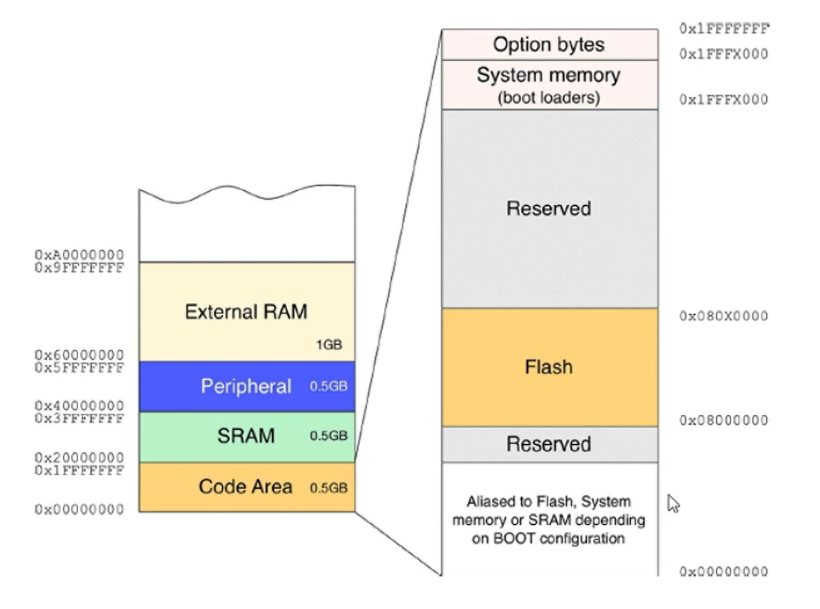
\includegraphics[scale=0.35]{Imagenes/stm/memoria2}\label{memo2}}
	\caption{Estructura de Memoria microcontroladores con Cortex M}
	\label{memoria}
\end{figure}

El espacio asignado como \textbf{Code Area} es aquel en el que se guardará el software que el programador escriba. Específicamente en la \textbf{Memoria Flash}. El bloque que lleva por nombre \textbf{System Memory} contiene el Boot Loader, el cual es una pieza de software que permite leer y escribir en la memoria flash sin necesidad de un interpretador (comúnmente llamado programador) como el St-Link V2 (Figura \ref{stlink}). El bloque superior llamado \textbf{Option Bytes} tiene particular interés puesto que gracias a estos bits podemos deshabilitar el acceso al software (guardado en la memoria flash) y así evitar una copia ilegal de nuestro software.

En el bloque \textbf{SRAM} es en donde se almacenan las variables. Los registros de configuración de perifericos se almacenan en \textbf{Perioheral} y los bloques \textbf{External Ram} y \textbf{External Device} nos dan la posibilidad de aumentar las capacidades del Microcontrolador en caso de ser necesario. Los tres bloque en la parte superior (figura \ref{memo1}) son bloque pertenecientes específicamente al microprocesador.


\begin{figure}[H]
	\centering
	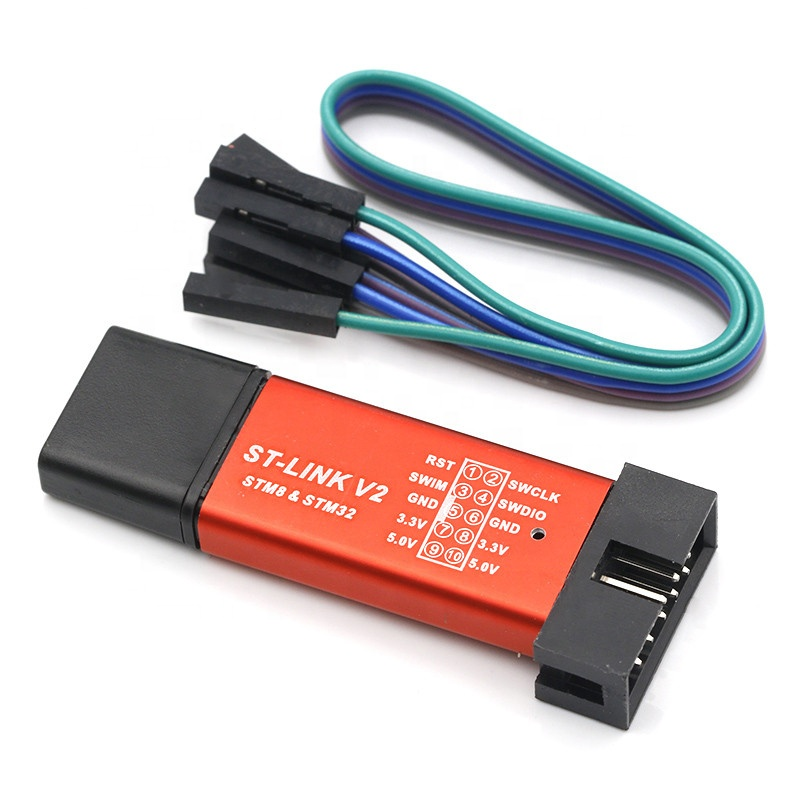
\includegraphics[scale=0.3]{Imagenes/stm/stlink}
	\caption{Interpretador (Programador)}
	\label{stlink}
\end{figure}

\section{Bit Masking - Bit Bandig}

\textbf{Bit Masking} tiene como propósito optimizar el uso de las variables. Y el \textbf{Bit Banding} en cambio, hace un uso poco eficiente de la memoria (es decir, desperdicia memoria) con el objetivo de optimizar las tareas del micro y el código en general.

De manera muy general, el bit banding es el proceso mediante el cual guardamos el valor de un bit en un registro y cuando saltamos a una interrupción y modificamos ese valor, lo que en realidad hacemos es operar con la dirección del registro donde guardamos el dato, motivo por el cual cuando regresamos de la interrupción ya tenemos el dato con los cambios hechos en la interrupción y podemos seguir operando.

Es decir que para cada bit que queramos resguardar usaremos un registro. Por este motivo se mencionó que es una técnica que desperdicia memoria.

Los registros que tienen esta finalidad los observamos en la siguiente imagen: 

\begin{figure}[H]
	\centering
	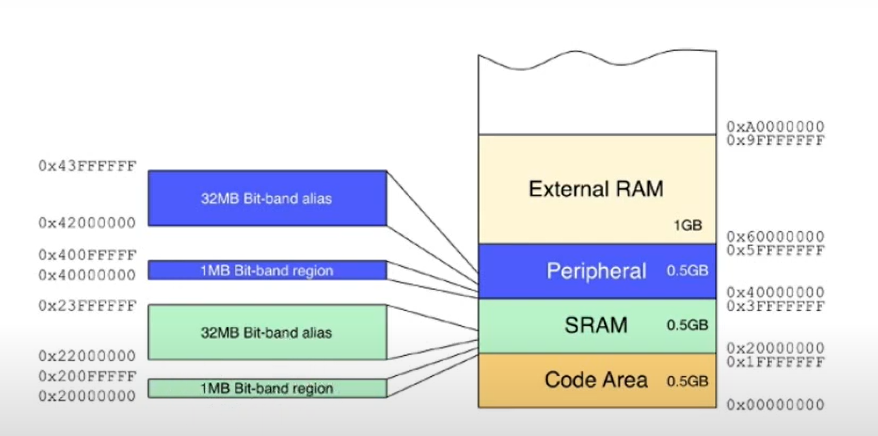
\includegraphics[scale=0.5]{Imagenes/stm/reg_banding}
	\caption{Registros dedicados a Bit Banding}
	\ref{banding}
\end{figure}

Pero hay que resaltar algo importante. Supongamos que en la interrupción el bit que quiero resguardar usando bit-banding pasa de ser un 1 a ser un 0. Cuando vuelvo de la interrupción puedo ejecutar una instrucción que sin que sea mi intención cambie el estado de ese bit, lo cual perdería sentido, se supone que el bit banding viene a solucionar estos casos. Este inconveniente se puede solucionar por software, pero los microcontroladores stm32 poseen un registro llamado \textbf{Registro de bloqueo} el cual es especial, puesto que no permite modificaciones como la antes presentada, por o cual el programador se aseguraría que el bit resguardado está protegido contra cambios accidentales.

\section{Instrucciónes THUMB-2}

Estas instrucciones son el resultado de la convinación de instrucción de 32 bits con instrucciones THUMB-16 (instrucciones de 16 bits). Las primeras desperdiciaba memoria y la segunda reducía la eficiencia del micro, entonces se desarrollaron las intrucciones nombradas en el título. Instrucciones que son usadas actualmente por microcontroladores cuyos procesadores sean Cortex M3, M4 o M7.

Algunas instrucciones son especiales, como las denominadas \textbf{VFP} (Vector Floating Point) que permiten operar con variables de punto flotante y las instrucciones \textbf{SIMD} cuyo tamaño puede llegar a ser 128 bits, estas son instrucciones que se ejecutan por múltiples procesadores. Es decir, una misma y unica instrucción ejecutada por dos o mas procesadores. El objetivo es, claramente, reducir tiempos lo que se traduce en un aumento de la eficiencia.

\section{Acceso no alineado y pipeline}

Acceso alineado y no alineado: 

\begin{figure}[H]
	\centering
	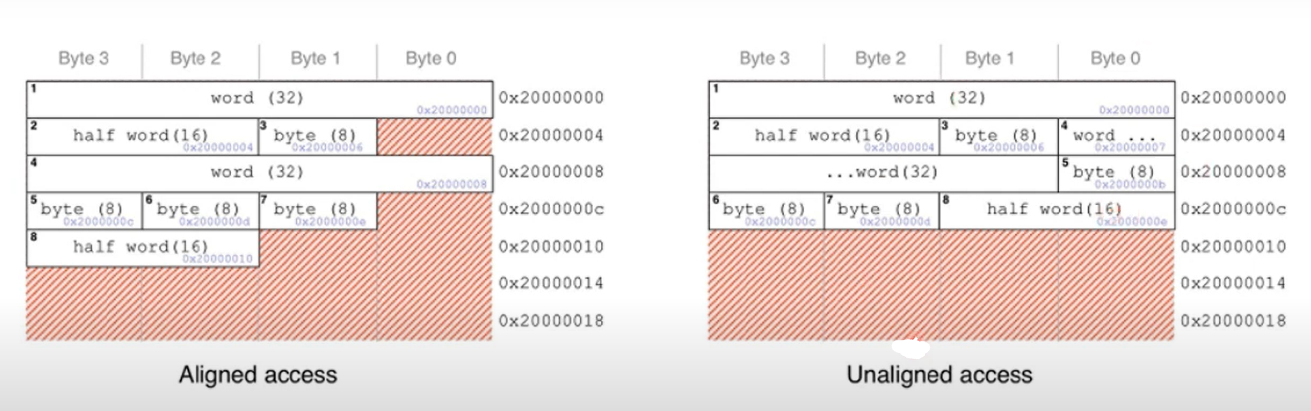
\includegraphics[scale=0.45]{Imagenes/stm/alignednotaligned}
	\caption{Acceso alineado y no alineado}
	\ref{memoacceso}
\end{figure}

Esto es una capacidad del procesador, no de la memoria.

 \subsection{Procesamiento de instrucciones}
 
 Al escribir un comando, el procesador deberá realizar una serie de \textbf{Instrucciones} para que la ejecución del comando sea efectiva. En general debe: Ubicar la instrucción $\rightarrow$ Decodificarla $\rightarrow$ Ejecutarla. Esto lleva su tiempo.
 
 \subsection{Pipeline}
 
Ejecución simultanea de instrucciones: 

\begin{figure}[H]
	\centering
	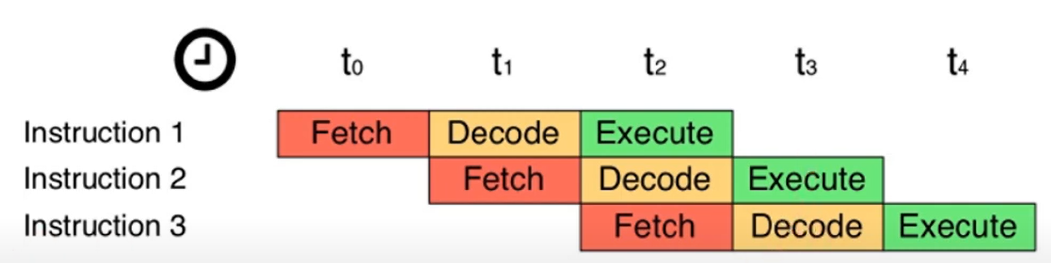
\includegraphics[scale=0.4]{Imagenes/stm/pipeline1}
	\caption{Ilustración de la técnica de Pipeline}
	\ref{pipe1}
\end{figure}


\section{Interrupciones y excepciones}

Las interrupciones y excepciones son rutinas (código) que se ejecutan cuando determinadas señales se presentan en el transcurso normal del código principal, de ahí el nombre interrupción y/o excepción.

La diferencia entre ellas es que a las interrupciones las activa un Hardware externo al micro y las excepciones son interrupciones propias del procesador.

Existe un periférico interno que se encarga de gestionar estas interrupciones, el ``Nested Vector Interrupt Controller'' (\textbf{NVIC}).

El código perteneciente a una interrupción se guarda en un espacio de memoria denominado ``Rutina de interrupción'' (\textbf{ISR}).

El código perteneciente a una Excepción se guarda en un espacio de memoria denominado ``Gestor de excepciones''.

Se las diferencia porque las primeras provienen del exterior del procesador y las excepciones en cambio provienen del mismo procesador. 

El procesador sabe donde buscar estos codigos (ya sean que pertenecen a una interrupción o a una excepción) gracias al \textbf{Vector Table}

Las excepeciones tienen distintas prioridades, prioridad que se representa con un numero, el cual mientras mas chico sea, mas prioridad tiene esa excepción. Por ejemplo, el ``Reset'' es una excepción con jerarquía -3, no hay otra que tenga mas jerarquía, pues nada puede frenar un reset, no tendria sentido que queramos resetear el micro y algo nos lo impida.
 
El modulo ``NVIC'' tiene algunas caracteristicas importantes de resaltar: 

\begin{itemize}
	\item No puede deshabilitar algunas excepciones como el Reset y el NMI.
	\item Es el periférico mediante el cual modificamos prioridades.
	\item Se encarga de ubicar el codigo de las interrupciones en la memoria flash.
	\item Permite el uso de memorias flash externa para guardar el codigo.
	\item Permite enmascarar fuentes de interrupciones, es decir, ocultar señales que disparan una interrupción.
\end{itemize}

Cuando las señales disparadoras de interrupciones vienen del exterior, son gestionadas por un periférico que se llama \textbf{External Interrupt Controller}, lo vemos en la figura \ref{bloques}. Cada Puerto del microcontrolador puede tener hasta 16 pines (por ejemplo PA0 a PA15, PB0 a PB15, etc), y cualquier pin puede ser usado como entrada de una señal de interrupción, pero al seleccionar uno de ellos, a los demas se los inhabilita para funcionar como entrada de una señal disparadora de interrupción. Es decir que si elijo por ejemplo el PA0, los demas PX0 no podran ser pines por donde ingrese una señal de interrupción. Se ve graficamente en la figura \ref{NVIC}.

\begin{figure}[H]
	\centering
	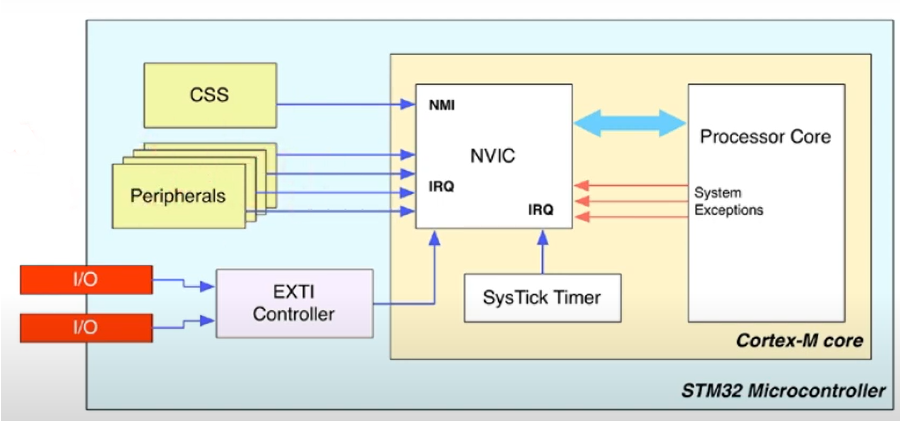
\includegraphics[scale=0.5]{Imagenes/stm/bloquesstm32}
	\caption{Diagrama microcontrolador}
	\label{bloques}
\end{figure}

\begin{figure}[H]
	\centering
	\includegraphics[scale=0.5]{Imagenes/stm/NVIC_interrup}
	\caption{Pines de interrupción}
	\label{NVIC}
\end{figure}

El código perteneciente a las interrupciones/Excepciones se encuentra en la memoria flash pero no con el código principal, tienen una ubicación especifica. Por este motivo existe algo que se denomina \textbf{Vector Table} el cual proporciona la información necesaria para que del código principal e procesador pueda ir a leer el código perteneciente a la interrupción que le corresponde hacer.

Un concepto muy importante en este tema es el \textbf{Pending Bit}. El cual es un bit que le avisa al NVIC que tiene una interrupción que atender. Por este motivo es muy importante que el programador lo desactive (mediante código) al salir de la interrupción (y lo activo al entrar) porque sino el NVIC interpretará que debe seguir ejecutando el código de la interrupción y nunca se detendrá.

\section{Systick Timer}


Timer especifico ubicado dentro del procesador. Su función es en relación a si usamos un RTOS o no. En el primer caso su trabajo es asignar una base periódica para las funciones. En el segundo caso asignará tiempos de ejecución, pues en el caso de no usarse RTOS las funciones se ejecutan hasta terminar y recién ahí se pasa a la siguiente.

\section{Interrupciones}

\subsection{Pasos para programar una interrupción}

\begin{enumerate}
	\item Configurar el pin como pin de interrupción y sus configuraciones electrónicas, (Niveles, Modos, etc).
	\item Activar el NVIC.
	\item Generar el código.
	\item En el \textbf{main.c} Abrir la función que configura los GPIO (\textbf{static void MX\_GPIO\_Init(void);}). Aquí verificamos solamente que las configuraciónes estén bien.
	\item Ir a Core $\rightarrow$ Inc $\rightarrow$ stm32f1xx\_it.h (o equivalente). Bajando vamos a encontrar los proptotipos de las funciones encargadas de gestionar la excepciones o interrupciones. Un ejemplo sacado del programa que prendia y apagaba el led segun puenteaba a masa un pin o no es: void EXTI9\_5\_IRQHandler(void);
	\item Abrir la función anterior. Dentro de esta función abrá otra del estilo: HAL\_GPIO\_EXTI\_IRQHandler(GPIO\_PIN\_9);
	\item Abrir esa función y ahí encontramos la función buscada: \textbf{Callback}.
	\item Copiamos la estructura (sin el \_weak) y la pegamos en el main.c, donde podremos programar dentro de ella la rutina que se ejecute cuando la interrupción se dispare.
\end{enumerate}
 
Si usamos varias interrupciones, el codigo irá dentro de la función \textbf{Callback}, pero tenemos que asegurarnos que se discriminen esas señales de interrupción. Como vemos en la figura \ref{interrupt}.

\begin{figure}[H]
	\centering
	\subfigure[Un solo pin de interrupción]{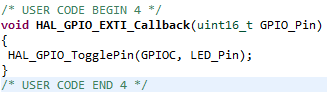
\includegraphics[scale=0.6]{Imagenes/stm/1interrupt} \label{I1}}
	\subfigure[2 Pines de interrupción]{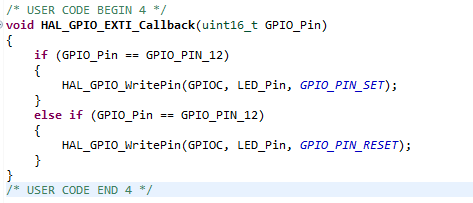
\includegraphics[scale=0.6]{Imagenes/stm/2interrupt}\label{I2}}
	\caption{Interrupciones}
	\label{interrupt}
\end{figure}

\subsection{Ciclo de vida de una interrupción}



\section{UART}

La utilización de la UART es simple gracias al entorno CubeIDE, solo se necesitan configurar los pines que son capaces de cumplir esa funcion y configurar los parametros (Baudrate, longitud de la palabra, sobremuestreo, etc).

Se puede utilizar la UART en modo de interrupción. Para esto tenemos disponibles dos funciones: 


\begin{itemize}
	\item HAL\_UART\_Transmit\_IT
	\item HAL\_UART\_Recive\_IT
\end{itemize}

Al tratarse de interrupciones, si hacemos una llamado a una función de las anteriores, comenzara a transmitir o recibir pero seguirá con otras instrucciones, no espera a final la transmisión o recepción.
Si llamamos dos veces seguidas a una función como las anteriores, la segunda será ignorada puesto que la UART estará ocupada, este es un punto a tener en cuenta porque puede traernos inconvenientes.


\subsection{Callbacks del UART}













\chapter*{Varios}

\textbf{10/09/20 Gino}
\begin{itemize}
	\item Reunión con Ing. Riva y Zerbini para definición de arquitectura.
	\item Solicitud de muestras gratis a Maxim (MAX2837, MAX5864).
\end{itemize}
\textbf{17/09/20 Gino}
\begin{itemize}
	\item Solicitud de muestra gratis a Qorvo (RFFC5071).
	\begin{figure}[H]
		\centering
		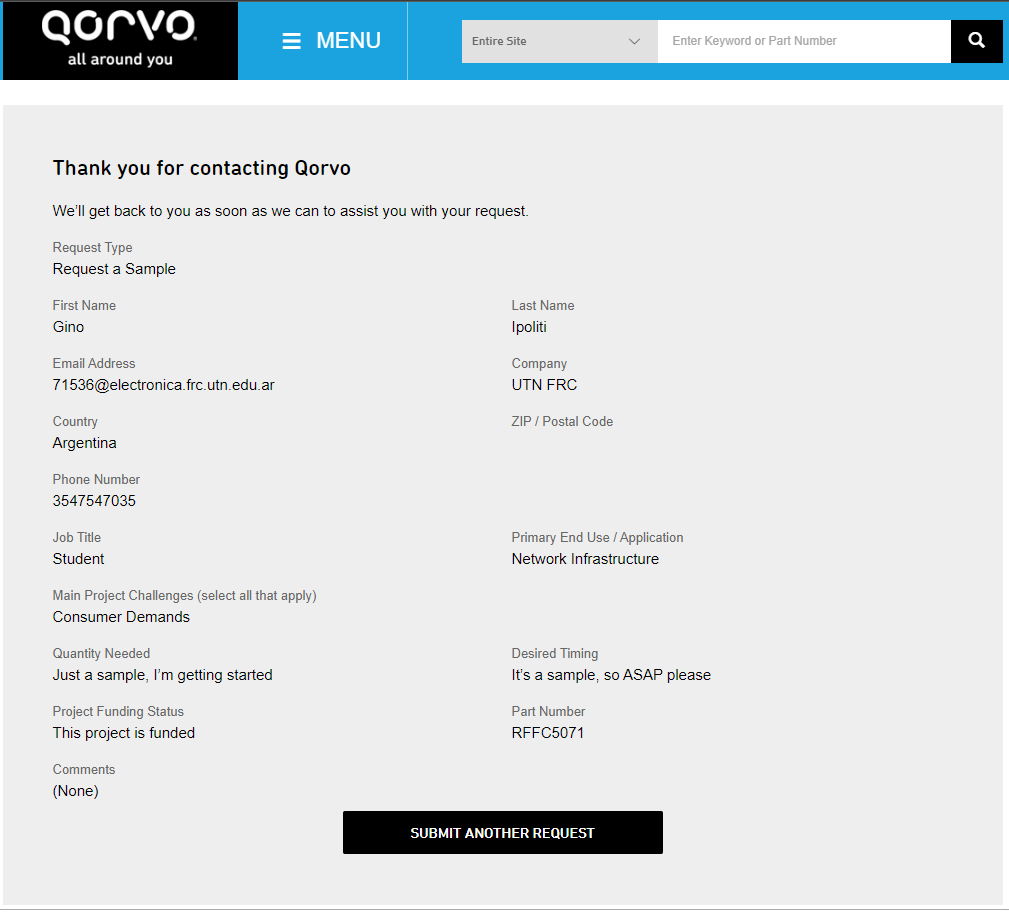
\includegraphics[scale=0.6]{Imagenes/sample_qorvo}
		\caption{Solicitud de sample}
	\end{figure}
\end{itemize}
\textbf{08/04/21 Gino}
\begin{itemize}
	\item Solicitud de muestra gratis a Renesas (generador de clock).
\end{itemize}






\bibliographystyle{IEEEtran}	
\bibliography{bibliografia}
\nocite{*}
\end{document}